%% LyX 2.4.0~beta5 created this file.  For more info, see https://www.lyx.org/.
%% Do not edit unless you really know what you are doing.
\documentclass[english]{foils}
\usepackage[T1]{fontenc}
\usepackage[latin9]{inputenc}
\pagestyle{foilheadings}
\setcounter{secnumdepth}{1}
\setcounter{tocdepth}{1}
\usepackage{xcolor}
\usepackage{array}
\usepackage{pifont}
\usepackage{amsmath}
\usepackage{amsthm}
\usepackage{amssymb}
\usepackage{graphicx}

\makeatletter

%%%%%%%%%%%%%%%%%%%%%%%%%%%%%% LyX specific LaTeX commands.
%% Because html converters don't know tabularnewline
\providecommand{\tabularnewline}{\\}
%% A simple dot to overcome graphicx limitations
\newcommand{\lyxdot}{.}


%%%%%%%%%%%%%%%%%%%%%%%%%%%%%% Textclass specific LaTeX commands.
\theoremstyle{definition}
\newtheorem{defn}{\protect\definitionname}
\newenvironment{lyxcode}
	{\par\begin{list}{}{
		\setlength{\rightmargin}{\leftmargin}
		\setlength{\listparindent}{0pt}% needed for AMS classes
		\raggedright
		\setlength{\itemsep}{0pt}
		\setlength{\parsep}{0pt}
		\normalfont\ttfamily}%
	 \item[]}
	{\end{list}}
\theoremstyle{definition}
\newtheorem*{example*}{\protect\examplename}

%%%%%%%%%%%%%%%%%%%%%%%%%%%%%% User specified LaTeX commands.
\usepackage{xcolor}
\renewcommand{\labelitemi}{$\textcolor{blue}{\bullet}$}
\renewcommand{\labelitemii}{$\textcolor{teal}{\Rightarrow}$}
\renewcommand{\labelitemiii}{$\textcolor{red}{\rightarrow}$}
\renewcommand{\labelitemiv}{$\textcolor{brown}{\circ}$}
% for French theorems, etc. since I'm using English to fix bullet pb.
\providecommand{\examplename}{Example}
\providecommand{\definitionname}{Definition}
\providecommand{\theoremnname}{Theorem}
\providecommand{\remarkname}{Remark}
\providecommand{\exercisename}{Exercise}
%
\graphicspath{{./graphics}}

\makeatother

\usepackage{babel}
\providecommand{\definitionname}{Definition}
\providecommand{\examplename}{Example}

\begin{document}

\MyLogo{Intro to ML}
\title{Probability and Statistics for Machine Learning}
\author{Mark Asch - IMU/VLP/CSU }
\date{2023}
\maketitle

\foilhead[-0.5in]{ML = STATISTICAL learning}
\begin{itemize}
\item all Machine Learning methods are statistical in nature, since we learn
general relationships from a sample/data/observations/measurements
\item in order to not just learn ``cooking recipes'', we will use a minimal
mathematical formalism that gives us a uniform and coherent representation
of statistical learning
\item we have:
\begin{itemize}
\item independent variables $x$ (inputs, features, attributes, explanatory
variables) 
\item dependent variables $y$ (outputs, responses, explained variables)
\item an unknown relationship, $f,$ that links inputs to outputs, and that
we want to learn from the available data
\begin{itemize}
\item for predictions
\item for inference
\end{itemize}
\end{itemize}
\end{itemize}

\foilhead{Populations and Samples}
\begin{defn}
A \textcolor{magenta}{population} is the set of all objects (observations)
being studied. Their number is denoted by $N$.
\end{defn}
~
\begin{defn}
A \textcolor{magenta}{sample} is a subset, of size $n,$ $n\le N,$
drawn from the population. We examine these observations to draw conclusions
and to make inferences about the population. 
\end{defn}
~

For \textcolor{magenta}{Big Data}:
\begin{dinglist}{56}
\item $N=$ALL ??? No.
\item Correlation $\Longrightarrow$ Causation ??? No.
\end{dinglist}

\foilhead{Pre-requisite: the mathematical framework}
\begin{itemize}
\item Suppose we have :

\begin{itemize}
\item a \textcolor{magenta}{response} variable (to explain), $Y$,
\item $p$ \textcolor{magenta}{explanatory,} variables, $X=(X_{1},X_{2},\ldots,X_{p})$,
\item $n$ \textcolor{magenta}{samples} of data, giving an $(n\times p)$
matrix, 
\[
X=\left[\begin{array}{cccc}
x_{11} & x_{12} & \cdots & x_{1p}\\
x_{21} & x_{22}\\
\vdots &  & \ddots\\
x_{n1} & x_{n2} & \cdots & x_{np}
\end{array}\right]
\]
\item a \textcolor{magenta}{relationship} between $Y$ and $X$ of the form
\[
Y=f(X)+\epsilon
\]
where

\begin{itemize}
\item $f$ is an \textcolor{magenta}{unknown} function of $X_{1},X_{2},\ldots,X_{p}$
\item $\epsilon$ is a random \textcolor{magenta}{error} term, independent
of $X,$ and with zero mean
\end{itemize}
\end{itemize}
\item ML is then an ensemble of approaches for \textcolor{magenta}{estimating}
$f$ with the objectsives of 

\begin{itemize}
\item \textcolor{magenta}{Prediction}: $\hat{Y}=\hat{f}(X)$ where $\hat{f}$
is an estimation for $f$ and $\hat{Y}$ is the resulting prediction
\item \textcolor{magenta}{Inference}: to understand how $Y$ varies as a
function of $X$ (correlations, importances, linearity, etc.)
\end{itemize}
\end{itemize}

\foilhead{Step 1: Exploratory Data Analysis (EDA)}
\begin{dinglist}{52}
\item An initial, \textcolor{magenta}{critical step }of the ``data science''
process
\item There are neither hypotheses, nor models - we \textcolor{magenta}{explore}
and we try to understand the problem!
\item The \textcolor{magenta}{tools} of EDA are :

\begin{itemize}
\item summary statistics
\item basic plots
\item graphics
\end{itemize}
\item The \textcolor{magenta}{methodology} : 

\begin{itemize}
\item systematic passage over all the data
\item plot all distributions of all the variables (``box plots'')
\item plot all the time series
\item try changes of variables (usually logs or powers)
\item look at all the relations two-by-two (``scatterplots'')
\item calculate all the summary statistics: mean, minumum, maximum, quartiles,
outliers
\end{itemize}
\end{dinglist}

\foilhead{SUMMARY Statistics }
\begin{itemize}
\item measures of
\begin{itemize}
\item central tendancy
\item dispersion around the centre
\end{itemize}
\end{itemize}

\foilhead{Measures of Central Tendancy}
\begin{itemize}
\item \textcolor{magenta}{mean}: 
\[
\bar{x}_{j}=\frac{1}{n}\sum_{i=1}^{m}x_{ij},\quad j=1,\ldots,p
\]
\end{itemize}
\begin{lyxcode}
\textcolor{teal}{>~Xj~~~~=~c(1,2,3,4,5)}

\textcolor{teal}{>~Xbarj~=~mean(Xj)}
\end{lyxcode}
\begin{itemize}
\item \textcolor{magenta}{median}: value for which at most the half of the
population is less than, and at least half is greater than, 
\[
\mathrm{median}(x)=\begin{cases}
x_{(n+1)/2}, & \mathrm{if}\,n\,\mathrm{odd}\\
\dfrac{x_{(n/2)}+x_{(n/2)+1}}{2}, & \mathrm{if}\,n\,\mathrm{even}
\end{cases}
\]
\end{itemize}
\begin{lyxcode}
\textcolor{teal}{>~Xmedj~=~median(Xj)}
\end{lyxcode}
\begin{itemize}
\item \textcolor{magenta}{mode}: the most frequent value (for which the
frequency/probability is maximal)
\end{itemize}

\foilhead{Measures of Dispersion}
\begin{itemize}
\item \textcolor{magenta}{variance} and standard deviation:
\[
s^{2}=\frac{1}{n-1}\sum_{i=1}^{n}\left(x_{i}-\bar{x}\right)^{2}
\]
\end{itemize}
\begin{lyxcode}
\textcolor{teal}{>~Xvar~=~var(Xj)}

\textcolor{teal}{>~Xstd~=~sd(Xj)}
\end{lyxcode}
\begin{tabular}{>{\raggedright}m{0.7\columnwidth}>{\centering}m{0.3\paperwidth}}
\begin{itemize}
\item \textcolor{magenta}{covariance} between $k$ variables, with $n$
observations each, is a $k\times k$ matrix with elements
\[
q_{jk}=\frac{1}{n}\sum_{i=1}^{n}\left(x_{ij}-\bar{x}_{j}\right)\left(x_{ik}-\bar{x}_{k}\right)
\]
\end{itemize}
\begin{lyxcode}
\textcolor{teal}{>~Xcov~=~cov(XX)~\#~covariance}

\textcolor{teal}{>~Xcor~=~cor(XX)~\#~correlation,~entre~-1~et~1}
\end{lyxcode}
 & 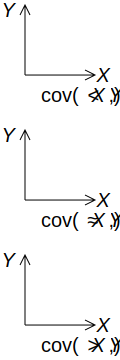
\includegraphics[scale=0.75]{graphics/Covariance_trends}\tabularnewline
\end{tabular}
\begin{itemize}
\item \textcolor{magenta}{quartiles}, quantiles and inter-quartile distance:
$z$ is the $k$-th $q$-quantile, if
\[
\Pr\left[X<z\right]\le\frac{k}{q}
\]

\begin{itemize}
\item the median is the second quartile, $Q_{2}$
\item la \textcolor{magenta}{inter-quartile distance }
\[
\mathrm{IQR}=Q_{3}-Q_{1}
\]
is a measure of dispersion 
\item the 100-quantiles are called \textcolor{magenta}{percentiles}
\end{itemize}
\end{itemize}
\begin{lyxcode}
\textcolor{teal}{>~range(Xj)~\#~max~-~min}

\textcolor{teal}{>~quantile(Xj)~\#~~0,~25,~50,~75~et~100\%}

\textcolor{teal}{>~IQR(Xj)}
\end{lyxcode}

\foilhead{Summary Statistics}
\begin{itemize}
\item the 5-number summary of Tukey is employed systematically for any data
analysis 
\begin{enumerate}
\item minimum
\item first quartile
\item median
\item third quartile
\item maximum
\end{enumerate}
\end{itemize}
\begin{lyxcode}
\textcolor{teal}{>~fivenum(Xj)}

\textcolor{teal}{>~summary(XX)}
\end{lyxcode}

\foilhead{Plots and Graphics for EDA}
\begin{itemize}
\item \textcolor{magenta}{box-plots}:
\end{itemize}
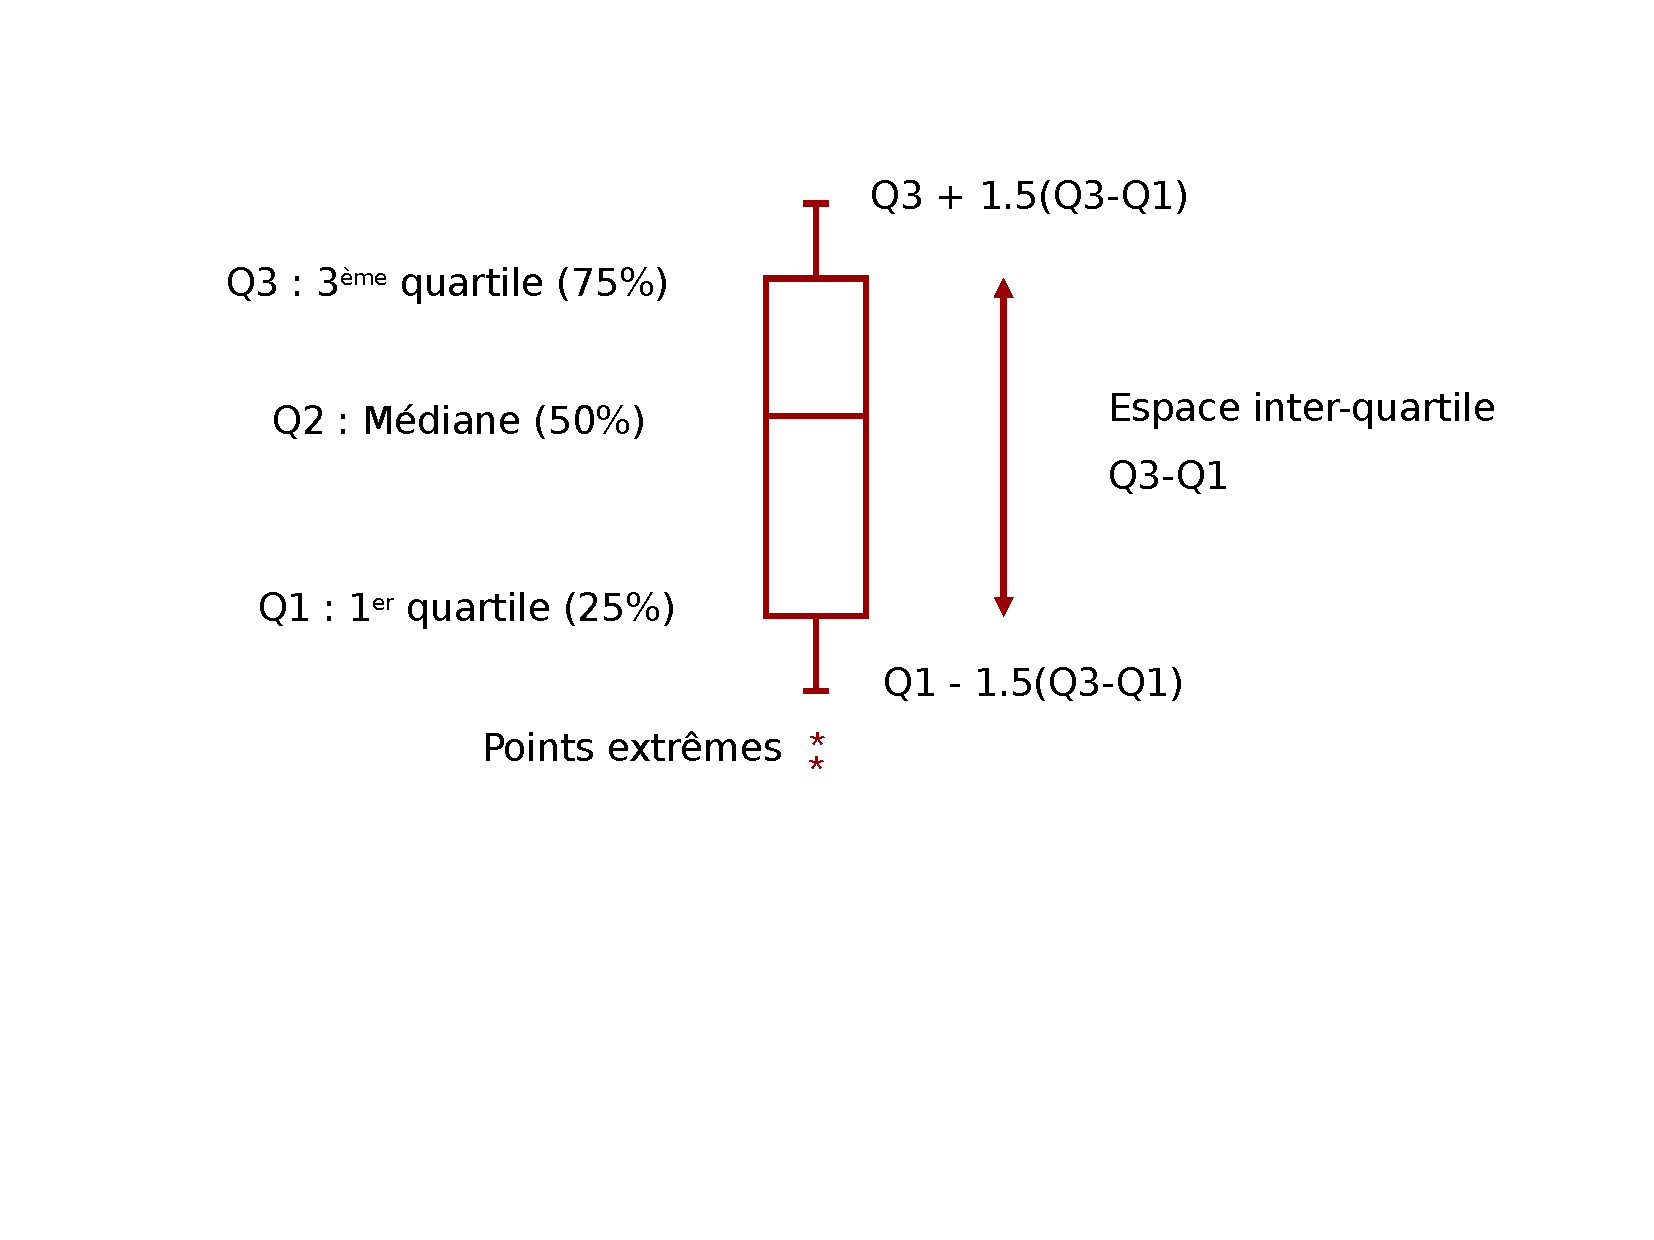
\includegraphics[width=1\columnwidth]{graphics/boxplot}
\begin{lyxcode}
\textcolor{teal}{>~boxplot(Xj)}
\end{lyxcode}
\begin{itemize}
\item \textcolor{magenta}{histograms}: 
\begin{itemize}
\item approximates the probability density function 
\item allows to detecti multi-modality...
\end{itemize}
\begin{lyxcode}
\textcolor{teal}{>~hist(Xj)}
\end{lyxcode}
\end{itemize}
\includegraphics[width=1\columnwidth]{graphics/Cumulative_vs_normal_histogram\lyxdot svg}

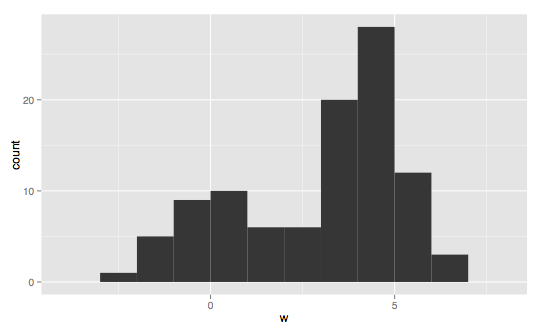
\includegraphics[width=0.6\textwidth]{graphics/Bimodal-histogram}
\begin{itemize}
\item \textcolor{magenta}{scatter-plots}: in the multi-variable case, allows
to display all the correlations, 2-by-2
\end{itemize}
\begin{lyxcode}
\textcolor{teal}{>~plot(XX)}
\end{lyxcode}
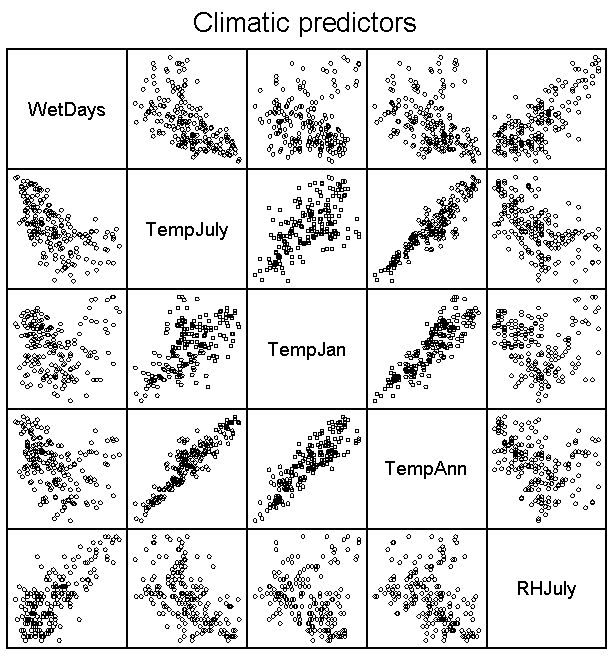
\includegraphics[totalheight=0.8\textheight]{graphics/NScatterplotMatrix}
\begin{itemize}
\item \textcolor{magenta}{q-q plots}: graphic of quantiles to verify the
hypothese of normality (Gaussian)
\end{itemize}
\begin{lyxcode}
\textcolor{teal}{>~qqnorm(Xj);~qqline(Xj)}
\end{lyxcode}
\includegraphics[width=0.8\textwidth]{graphics/1024px-Normal_normal_qq\lyxdot svg}

\foilhead{Significance and Covariates}
\begin{itemize}
\item the 2 fundamental notions for \textcolor{magenta}{UNDERSTANDING} any
statistical model
\begin{itemize}
\item significance (bad!) and confidence intervals (better)
\item covariates need to be chosen judiciously (can produce false significance)
\end{itemize}
\end{itemize}

\foilhead{Significance Tests }
\begin{example*}
Compare a new and an old treatment against hypertension.
\end{example*}
\begin{itemize}
\item suppose the data \textbf{seem} to indicate that the new treatment
is better
\item can we exclude a sampling <<accident>>, where the new treatment
was given almost exclusively to subjects in good health???
\item the significance test would state that this result is very unlikely
(small value of $p$) under the null hypothesis (= no effect)
\item Conclusion (dangerous!): the two treatments have a \textcolor{magenta}{significant}
diffference at level $\alpha$ ($>p$).
\end{itemize}

\foilhead{Significance Tests : conclusion}
\begin{itemize}
\item significance tests should be avoided (official recommendation of the
ASA in 2016)
\begin{itemize}
\item at worst, they are misleading
\item at best, they are uninformative
\end{itemize}
\item producing a \textcolor{magenta}{confidence interval} (point estimate
+/- error margin) is much better
\begin{itemize}
\item usually, at a 95\% level
\item ``in 95\% of all possible samples, the empirical estimate will lie
within the error margin of the true value of the population''
\item however, we will not repeat the sampling numerous times---this is
ususally impossible... hence the interest of Bayesian approaches...
(TBC)
\end{itemize}
\end{itemize}

\foilhead{Explanatory Variables}
\begin{itemize}
\item we study the relationship between a variable $Y$ and a variable $X$
\end{itemize}
\begin{example*}
Evaluation in 4 hospitals of survival rates after a heart attack
\end{example*}
\begin{itemize}
\item let the response $Y=1$ if the patient survives, $Y=0$ if not.
\item let $X=1,\ldots,4$ be the identifier of the hospital
\item measuring the relationship between $Y$ and $X$ implies here to compare
the 4 hospitals in terms of the survival rate...
\begin{itemize}
\item but 1 of the 4 hospitals serves a zone with a large proportion of
old patients
\item so a direct comparison would be unfair, and inexact...
\end{itemize}
\item we need to introduce a new explanatory variable , $Z=\mathrm{age}$
and measure the relationship between $Y$ and $X$ keeping $Z$ constant
(or by age intervals)
\item a correlation can pass from positive to negative (change of sign)
once the covariate $Z$ is taken into account
\begin{itemize}
\item Simpson's paradox..
\item related to \textcolor{magenta}{causality}! (TBC)
\end{itemize}
\end{itemize}

\foilhead{Cross Validation }
\begin{itemize}
\item an ensemble of techniques for testing the \textcolor{magenta}{predictive
power} of a statistical learning model
\item indispensable step for validating the \textcolor{magenta}{robustness}
of a model
\begin{itemize}
\item avoids the ``good luck'' effect 
\end{itemize}
\item also possible to propose \textcolor{magenta}{confidence intervals }
\begin{itemize}
\item using the ``bootstrap''
\end{itemize}
\end{itemize}

\end{document}
